\documentclass[convert={density=900,size=1080x800,outext=.png}]{standalone}
\usepackage{tikz}

\usetikzlibrary{calc, positioning}
\usetikzlibrary{arrows.meta}
\usetikzlibrary{matrix}
\usetikzlibrary{shadows}
\usepgflibrary{shapes.misc}
\usepgflibrary{{shapes.geometric}}

\pgfdeclarelayer{shadow} 
\pgfsetlayers{shadow,main}
\def\shadowradius{3pt}


\def\mw{1.5cm}
\def\mh{1.25cm}

\tikzstyle{component} = [draw, fill=white, minimum width=\mw, minimum height=\mh, align=center]

\tikzset{
    border/.style = { 
        draw, rectangle, minimum width=\mw, minimum height=\mh, thick, align=center, ultra thick
    },
    Component/.pic = {
        \node [border](-edge){#1}; 
    },
}

\tikzset{
    clockborder/.style = { 
        trapezium, trapezium angle=60, minimum width=1cm, draw, very thick
    },
    Clock/.pic = {
        \node [clockborder, shape border rotate=-180](-clockedge){#1};
        \draw[very thick] (-clockedge.east) -- ++(2cm, 0cm);
        \def\sft{0.5}
        \foreach \x in {0, 0.5, 1, 1.5}{
            \draw[very thick] (\x + \sft, 0.1) -| ++(0.25cm, 0.25cm) -| ++ (0.25cm, -0.25cm);
        }
    },
}

\begin{document}
    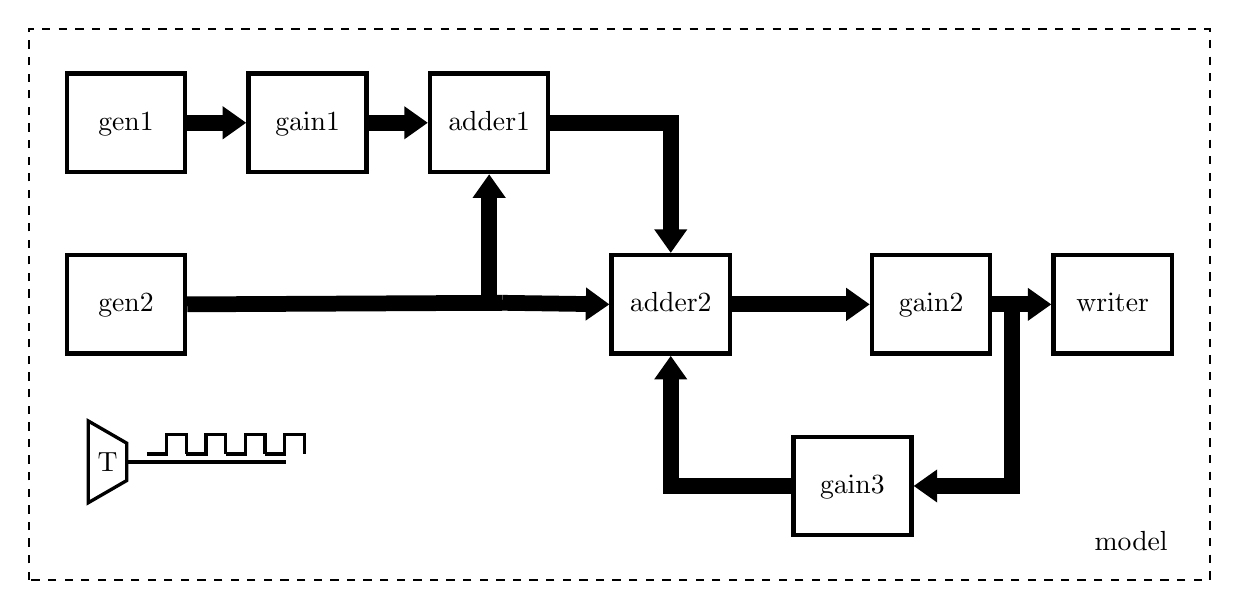
\begin{tikzpicture}
        % Place the blocks 
        \matrix (m) [
            matrix of nodes, 
            ampersand replacement=\&, 
            column sep = 0.75cm, 
            row sep = 1cm, 
            nodes={
                text height=1.5ex,
                text depth=.25ex,
                anchor=center}
                ]{
                    \draw pic (gen1) {Component={gen1}}; \& \draw pic (gain1) {Component={gain1}}; \& \draw pic (adder1) {Component={adder1}}; \& 
                                         \&                                  \&                                  \\
                    \draw pic (gen2) {Component={gen2}}; \&                                  \&                                  \& 
                    \draw pic (adder2) {Component={adder2}}; \& \draw pic (gain2) {Component={gain2}}; \& \draw pic (writer) {Component={writer}}; \\
                                         \&                                  \&                                  \& 
                                         \& \draw[xshift=-1cm] pic (gain3) {Component={gain3}}; \&                                  \\
                };

        % Draw connections 
        \begin{scope}[line width=2mm, >={Triangle[width=4mm,length=3mm]}]
            \def\shiftamount{0.5mm};
            \draw[->] (gen1-edge.east) -- (gain1-edge.west);
            \draw[->] (gain1-edge.east) -- (adder1-edge.west);
            \draw[->] (adder1-edge.east) -| (adder2-edge.north);
            \draw[-] (gen2-edge.east) -- ++ (4cm, 0.02cm) coordinate(a);
            \draw[->] (a) -| (adder1-edge.south);
            \draw[->] (a) -- (adder2-edge.west);
            \draw[->] (adder2-edge.east) -- (gain2-edge.west);
            \draw[-] (gain2-edge.east) -- ++ (0.25cm, 0.0cm) coordinate(b);
            \draw[->] (b) |- (gain3-edge.east);
            \draw[->] (b) |- (writer-edge.west);
            \draw[->] (gain3-edge.west) -| (adder2-edge.south);
        \end{scope}

        % \Place clock 
        \begin{scope}[shift={(-6.5cm, -2cm)}]
            \draw pic(clk) {Clock={T}} ;
        \end{scope}

        %  Draw rectangle 
        \draw[dashed, thick] (-7.5, -3.5) rectangle (7.5, 3.5);
        \draw (0,0) node[yshift=-3cm, xshift=6.5cm]{model};
    \end{tikzpicture}
\end{document}